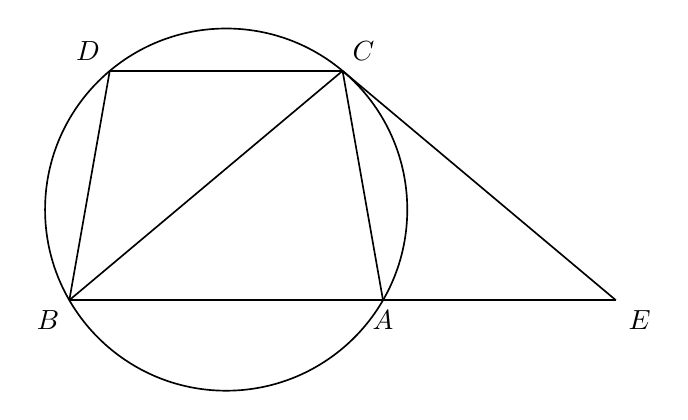
\begin{tikzpicture}[x=1cm,y=1cm,line width=.6pt,font=\normalsize]
\coordinate (O) at (0,0);
\coordinate (B) at (-1.9919,-1.15);
\coordinate (A) at (1.9919,-1.15);
\coordinate (C) at (1.4784,1.7619);
\coordinate (D) at (-1.4784,1.7619);
\coordinate (E) at (4.9487,-1.15);
\draw[black] (O) circle[radius=2.3cm];
\draw[black] (B)--(E);
\draw[black] (D)--(C);
\draw[black] (D)--(B);
\draw[black] (C)--(A);
\draw[black] (B)--(C);
\draw[black] (C)--(E);
\node[below left] at (B) {$B$};
\node[below] at (A) {$A$};
\node[below right, xshift=1pt] at (E) {$E$};
\node[above right] at (C) {$C$};
\node[above left] at (D) {$D$};
\end{tikzpicture}
